
%%%%%%%%%%%%%%%%%%%%%%%%%%%%%%%%%%%%%%%%%%%%%%%%%%%%%%%%%%%%%%%%%%%%%%%%%%%%%%%%%%%%%%%%%%%%%%%%%
%
% Document:      DP  organisation chart reporting lines
%
%%%%%%%%%%%%%%%%%%%%%%%%%%%%%%%%%%%%%%%%%%%%%%%%%%%%%%%%%%%%%%%%%%%%%%%%%%%%%%

\documentclass{article}

\usepackage{times,layouts}
\usepackage{tikz,hyperref,amsmath}
\usetikzlibrary{positioning,arrows,shapes,decorations.shapes,shapes.arrows}
\usetikzlibrary{backgrounds,calc}

\usepackage[paperwidth=28cm,paperheight=16.0cm,
left=-2mm,top=3mm,bottom=0mm,right=0mm,
noheadfoot,marginparwidth=0pt,includemp=false ]{geometry}


\newcommand\showpage{%
\setlayoutscale{0.5}\setlabelfont{\tiny}\printheadingsfalse\printparametersfalse
\currentpage\pagedesign}

\hypersetup{pdftitle={DM organisation }, pdfsubject={Diagram illustrating the
 reporting lines in LSST DM Group}, pdfauthor={ William O'Mullane}}


%%%%%%%%%%%%%%%%%%%%%%%%%%%%%%%%%%%%%%%%%%%%%%%%%%%%%%%%%%%%%%%%%%%%%%%%%%%%%%%%%%%%%%%%%%%%%%%%%
%
% Document:      Boxes and lines for all diagrams
%
%%%%%%%%%%%%%%%%%%%%%%%%%%%%%%%%%%%%%%%%%%%%%%%%%%%%%%%%%%%%%%%%%%%%%%%%%%%%%%

\tikzstyle{divbox}=[rectangle, rounded corners=3pt, draw=blue, top color=blue!30!white, bottom
color=white, very thick, minimum height=12mm, inner sep=3pt, text centered, text width=35mm]

\tikzstyle{arcbox}=[rectangle, rounded corners=3pt, draw=red, top color=yellow!50!white, bottom
color=white, very thick, minimum height=12mm, inner sep=2pt, text centered, text width=50mm]

\tikzstyle{psbox}=[rectangle, rounded corners=3pt, draw=red, top color=green!50!white, bottom
color=cyan, very thick, minimum height=10mm, inner sep=2pt, text centered, text width=35mm]

\tikzstyle{pobox}=[rectangle, rounded corners=3pt, draw=red, top color=blue!50!white, bottom
color=cyan, very thick, minimum height=10mm, inner sep=2pt, text centered, text width=35mm]

\tikzstyle{docbox}=[rectangle, rounded corners=3pt, draw=black, fill=cyan!50!white, 
 very thick, minimum height=12mm, inner sep=2pt,  text centered, text width=30mm]

\tikzstyle{docboxm}=[rectangle, rounded corners=3pt, draw=black, fill=red!50!white, 
 very thick, minimum height=12mm, inner sep=2pt,  text centered, text width=30mm]

\tikzstyle{docboxicd}=[rectangle, rounded corners=3pt, draw=black, fill=green!70!white, 
 very thick, minimum height=12mm, inner sep=2pt,  text centered, text width=30mm]

\tikzstyle{gbox}=[rectangle, rounded corners=3pt, draw=orange!80!black, top color=orange!30!white,
bottom color=white, very thick, minimum height=12mm, inner sep=5pt, text badly ragged, text width=40mm]

\tikzstyle{mbox}=[rectangle, rounded corners=3pt, draw=blue, top color=cyan!50!white, bottom
color=white, very thick, minimum height=8mm, inner sep=2pt, text centered, text width=30mm]

\tikzstyle{line}=[-, thick]
\tikzstyle{sline}=[-, thick, dashed, olive]
\tikzstyle{dline}=[->, thick, cyan]
\tikzstyle{tline}=[->, thick, dashed, blue]
\tikzstyle{pline}=[->, thick,  black!60!white]

\xdefinecolor{softviolet}{rgb}{0.85, 0.8, 1.0}




\begin{document}

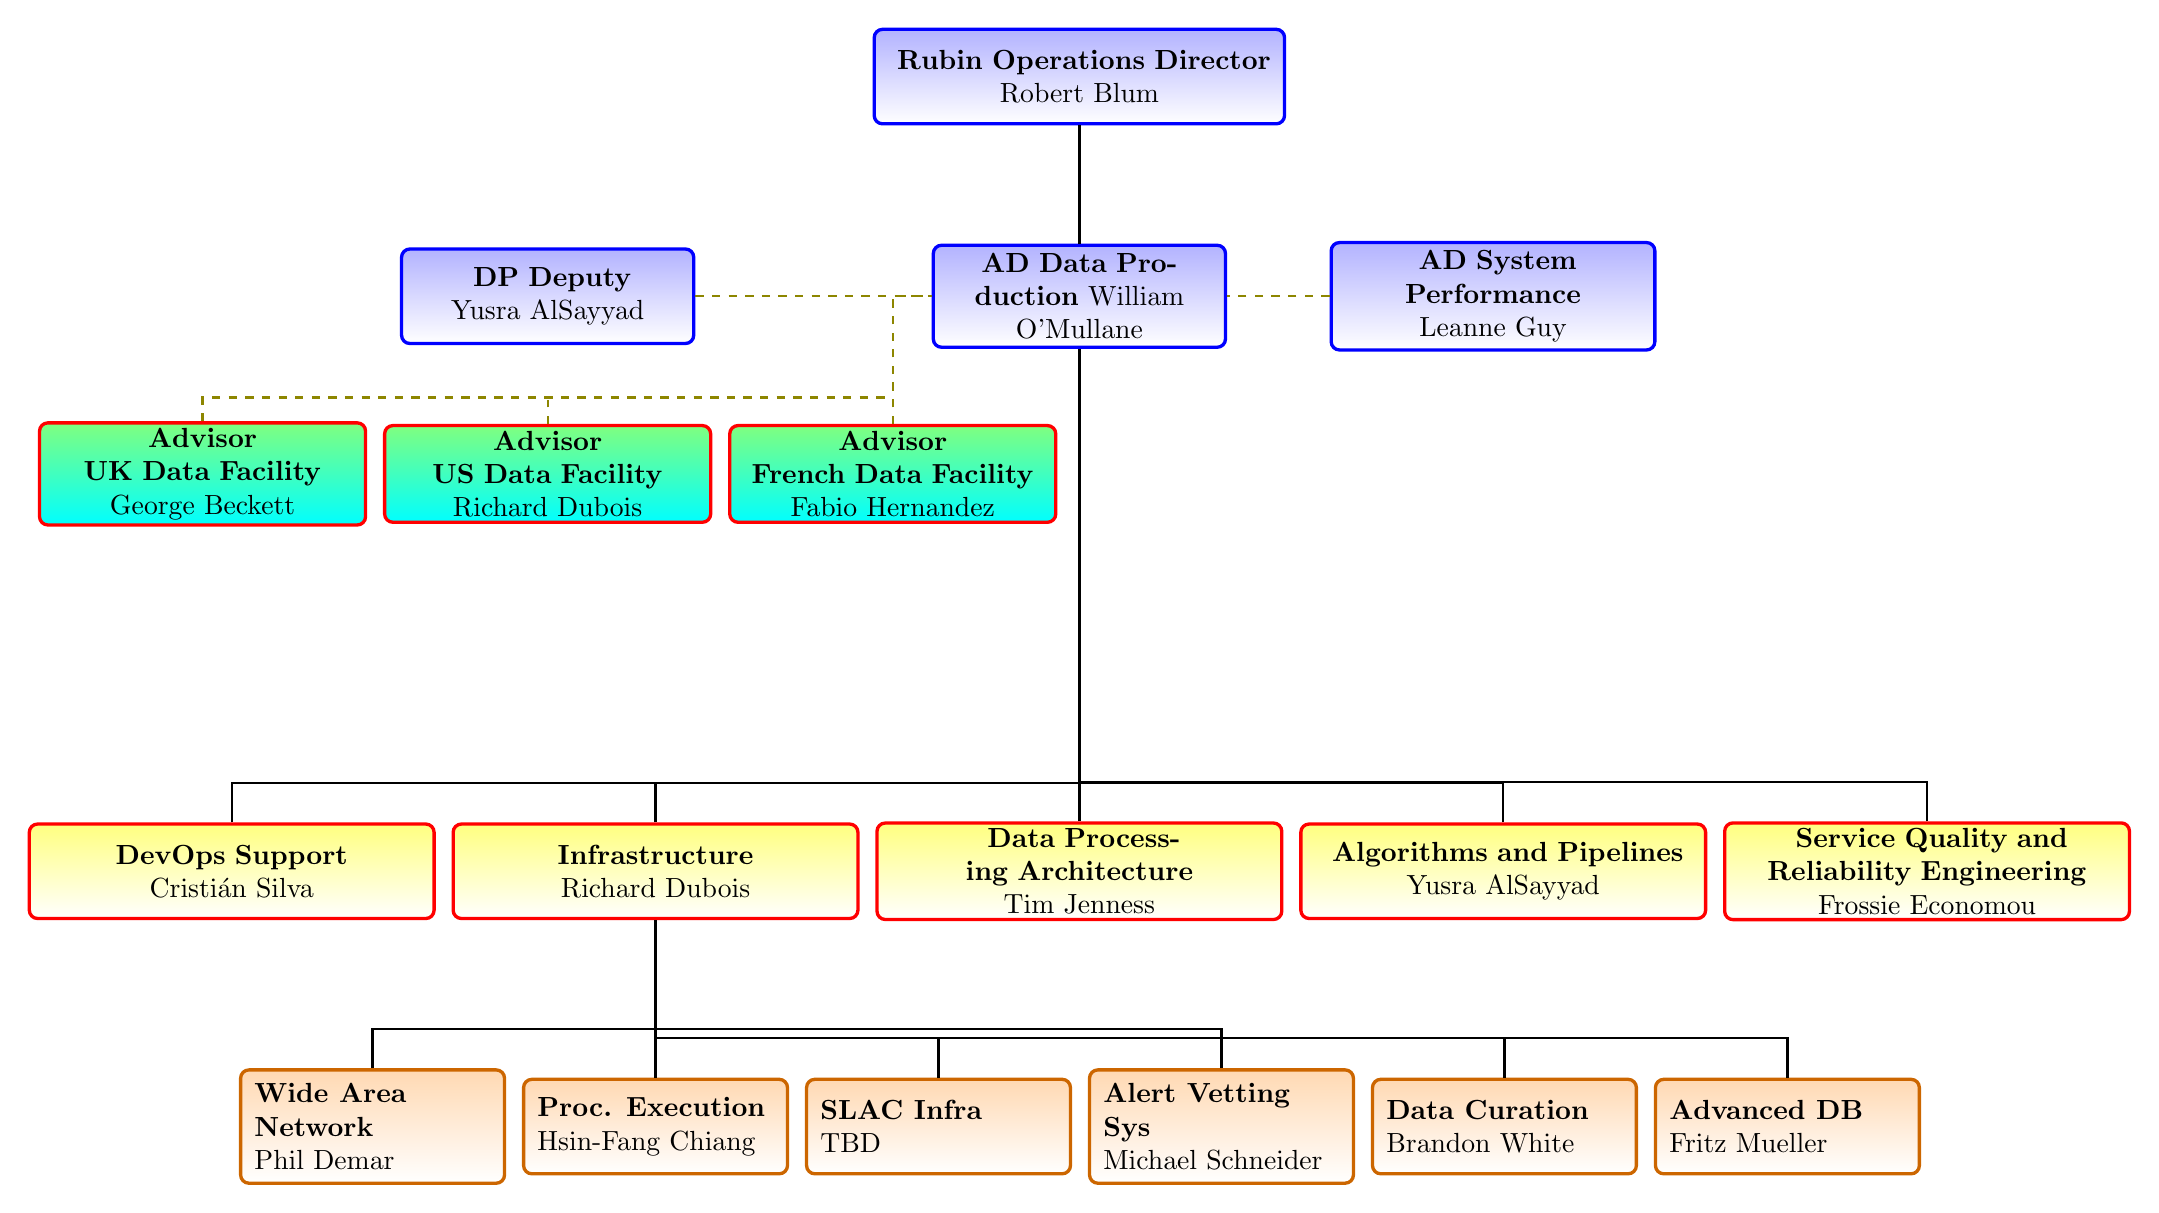
\begin{tikzpicture}[node distance=0mm]


    \node (dpad) [divbox] {\textbf{AD Data Production} William O'Mullane};
    \node (ddpad) [divbox, left=3cm of dpad] {\textbf{ DP Deputy } \\Yusra AlSayyad};
    \node (dir) [divbox, above=1.5cm of dpad, text width=5cm] {\textbf{ Rubin Operations Director} \\Robert Blum };
    \node (spad) [divbox, right=1.3cm of dpad, minimum height=12mm, text width=39mm] {\textbf{ AD System Performance}\\ Leanne Guy };
    %\node (dspad) [psbox, right=0.4cm of dmps, minimum height=12mm, text width=41mm] {\textbf{ SP Deputy }\\ Colin Slater };
    %\node (ps) [psbox, right=1.5cm of pm, minimum height=12mm] {\textbf{  Project Scientist}\\ \u{Z}eljko Ivezi\'c};

    \node (udfa) [psbox, below=1cm of ddpad, text width=4cm] {\textbf{Advisor \\US Data Facility}\\ Richard Dubois };
    \node (fdfa) [psbox, right=0.2cm of udfa, text width=4cm] {\textbf{Advisor \\French Data Facility}\\ Fabio Hernandez};
    \node (ukfa) [psbox, left=0.2cm of udfa, text width=4cm] {\textbf{Advisor \\UK Data Facility}\\ George Beckett };
    %\node (udpad) [below=61mm of dpad, text width=0mm]{};

%
	%\node(tfl)[arcbox,below=2cm of spad.west]{\textbf{ DP0 Task Force Lead} \\Hsin-Fang Chiang } ;
	\node(sumw)[arcbox,below=6cm of dpad]{\textbf{ Data Processing Architecture} \\Tim Jenness} ;
	\node(alp)[arcbox,right=2mm of sumw]{\textbf{ Algorithms and Pipelines } \\Yusra AlSayyad} ;
	\node(spare)[arcbox,right=2mm of alp]{\textbf{ Service Quality and Reliability Engineering } \\Frossie Economou} ;
	\node(infra)[arcbox,left=2mm of sumw]{\textbf{Infrastructure} \\ Richard Dubois} ;
	\node(devops)[arcbox,left=2mm of infra]{\textbf{DevOps Support} \\ Cristi\'{a}n Silva} ;
	\node(exec)[gbox,text width=30mm,below=2cm of infra]{\textbf{Proc. Execution} \\ Hsin-Fang Chiang} ;
	\node(wan)[gbox,text width=30mm,left=2mm of exec]{\textbf{Wide Area Network} \\ Phil Demar} ;
	\node(sinfra)[gbox,text width=30mm,right=2mm of exec]{\textbf{SLAC Infra} \\ TBD } ;
	\node(avs)[gbox,text width=30mm,right=2mm of sinfra]{\textbf{Alert Vetting Sys} \\ Michael Schneider } ;
	\node(datac)[gbox,text width=30mm,right=2mm of avs]{\textbf{Data Curation} \\ Brandon White } ;
	\node(adb)[gbox,text width=30mm,right=2mm of datac]{\textbf{Advanced DB} \\ Fritz Mueller } ;
%Lines ..

   \draw[line] (dpad.north) -- ++(0,0.8) -| (dir.south);
   \draw[sline] (ddpad.east) --  (dpad.west);

%dm lines second number is the proportional turning point of the line
%\draw[line] (tfl.west)  -| (dpad.south);
   \draw[line] (sumw.north) --  (dpad.south);
\draw[line] (spare.north)-- ++(0,0.5)  -| (dpad.south);
\draw[line] (alp.north) -- ++(0,0.5) -| (dpad.south);
\draw[line] (infra.north)-- ++(0,0.5) -| (dpad.south);
\draw[line] (devops.north)-- ++(0,0.5)  -| (dpad.south);

  \draw[line] (exec.north) --  (infra.south);
\draw[line] (wan.north)-- ++(0,0.5)  -| (infra.south);
\draw[line] (adb.north)-- ++(0,0.5)  -| (infra.south);
\draw[line] (datac.north)-- ++(0,0.5)  -| (infra.south);
\draw[line] (sinfra.north)-- ++(0,0.5)  -| (infra.south);
\draw[line] (avs.north)-- ++(0,0.5)  -| (infra.south);
%science
\draw[sline] (spad.west) to (dpad.east);
\draw[sline] (fdfa.north) |-  (dpad.west);
\draw[sline] (udfa.north) |- ++(0,0.3) ;
\draw[sline] (ukfa.north) |- ++(0,0.3) -- ++(8.7,0) ;



\end{tikzpicture}
\end{document}
